\subsection{Architektur}
\label{subsec:architecture}

Die Entwicklung eines Softwaresystem ist ein komplexes Unterfangen und oft nicht mehr überschaubar.
Daher wollen wir bei der Darstellung der Architektur auf einer Makroebene beginnen und nachfolgend einige Details beleuchten.
Am Ende soll dadurch ein detailliertes Verständnis der Anwendung möglich sein.

\subsubsection{Makrosicht}
\label{subsubsec:macro-view}

Unter der Makrosicht der Architektur, wie in Abbildung~\ref{fig:macro-view-diagram} dargestellt, verstehen wir eine grobe Ansicht der verwendeten Komponenten des Softwaresystems.

\begin{figure}[h]
    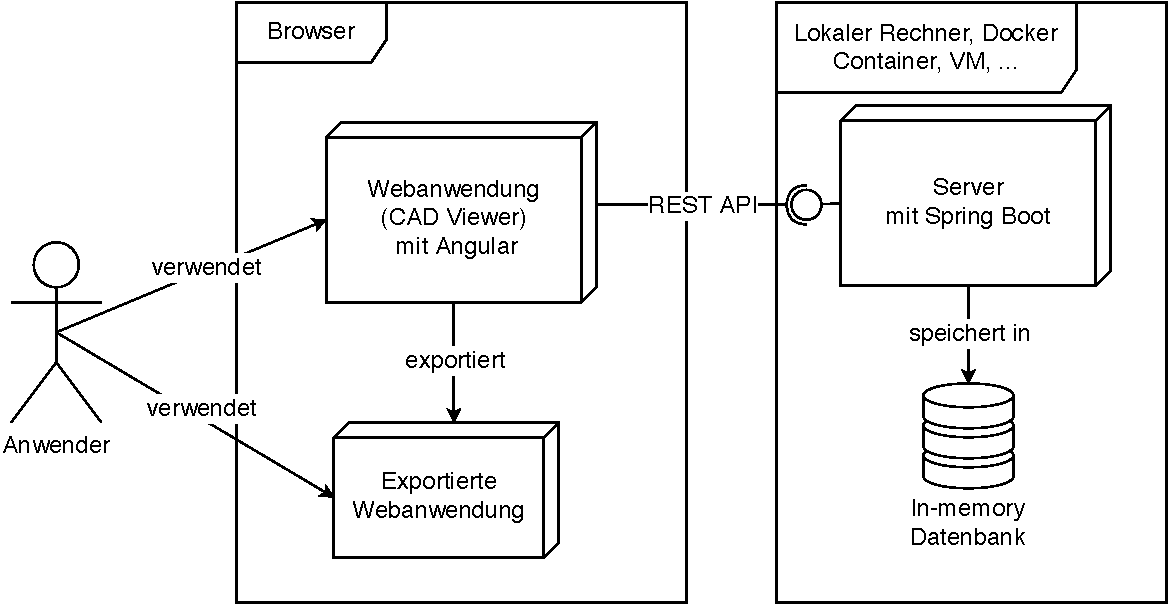
\includegraphics[width=0.5\textwidth]{res/macro.pdf}
    \caption{Darstellung der Makrosicht der Anwendungsarchitektur.}
    \label{fig:macro-view-diagram}
\end{figure}

Die Kernanwendung, der CAD-Viewer, läuft als Webanwendung auf dem Browser des Anwenders.
Wir haben uns dazu entschieden, dass die Exportfunktion wiederum dieselbe Webanwendung, nur ohne Serveranbindung und mit eingebetteter CAD-Datei, exportiert.
Daher befindet sich die exportierte Webanwendung ebenso im Bereich des Browsers.

Auf der anderen Seite des Diagramms ist die Serveranwendung zu finden, welche über eine REST-API angesprochen wird.
Der Server stellt neben seinen Schnittstellen auch die Webanwendung bereit.
Ebenso ist eine In-memory Datenbank darunter dargestellt, auf welcher die hochgeladenen CAD-Dateien und Raumzuordnungen flüchtig gespeichert werden.
Wir haben uns für eine flüchtige Speicherung entschieden, da aus unserer Sicht kein Mehrwert durch die Persistierung entstünde.
Nichtsdestotrotz kann die verwendete Datenbank auch im Nachhinein mittels Kommandozeilenparameter wie \texttt{--spring.datasource.url} umkonfiguriert werden, um so auch nicht-flüchtige Datenbanken anzubinden~\cite{JDBCSpringBoot}.

Während die Webanwendung klar im Browser des Anwenders läuft, ist das Laufzeitsystem des Servers unbestimmt.
Es kann sich dabei beispielsweise um den lokalen Rechner eines Anwenders handeln, eine VM oder eine Docker Container.

\subsubsection{Detailsicht des Servers}
\label{subsubsec:detail-server}

Nach dieser ersten groben Ansicht gehen wir zunächst näher auf den Server ein.
Wie bereits erwähnt handelt es sich um eine Java-Anwendung auf Basis des Spring Frameworks.
Der primäre Zweck ist die Bereitstellung einer REST-API zum Hochladen und Verwalten von CAD-Dateien und Raumzuordnungen.
Zwar ließe sich die Darstellung und der Raumzuordnungsvorgang auch direkt in der Webanwendung abhandeln, jedoch ermöglicht die API eine schnellere und automatisierte Bereitstellung der CAD-Dateien und Raumzuordnungen.
So können beispielsweise die Clusteringergebnisse und dazugehörigen Gebäudepläne bereits automatisch nach dem Clustering über ein Python-Skript - oder Ähnliches - hochgeladen werden, ohne manuell jede Datei einzeln über die Webanwendung auswählen zu müssen.
Die Webanwendung kann die API verwenden, um die bereits hochgeladenen Dateien einzusehen und bei Bedarf herunterzuladen.
Außerdem hat der Server noch die Funktion den Export der Webanwendung auszuführen, die er selbst bereitstellt.

\begin{figure}[h]
    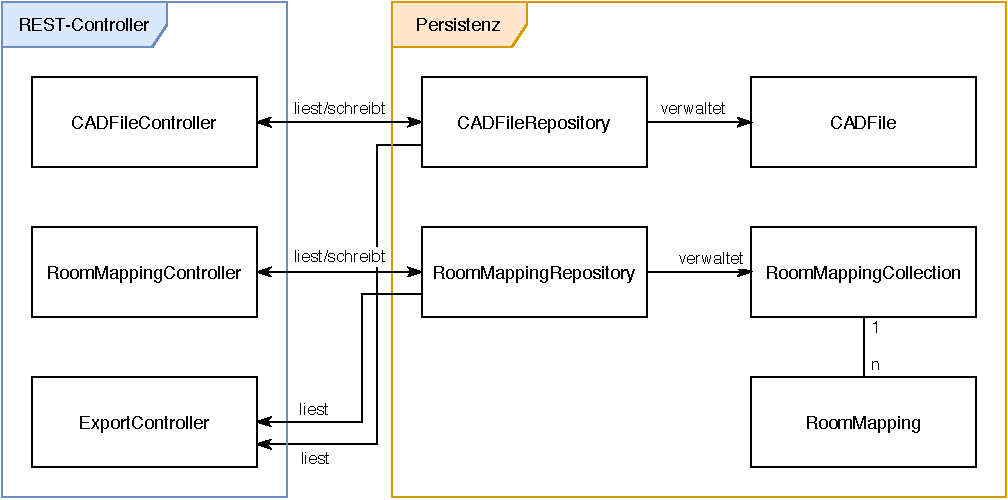
\includegraphics[width=0.55\textwidth]{res/server-architecture.pdf}
    \caption{Darstellung der Detailansicht der Serveranwendung.
    Dabei sind die REST-Controller, welche die REST-API abbilden sowie die Persistenzschicht abgebildet.}
    \label{fig:detail-view-server}
\end{figure}

Wir haben ein Diagramm des Feinentwurfs der Serveranwendung in Abbildung~\ref{fig:detail-view-server} dargestellt.
Zur Linken sind dabei die REST-Controller zu finden, also Komponenten, die in einer Spring Anwendung die REST-API abbilden.
Wir stellen dabei Schnittstellen zur Verwaltung von CAD-Dateien, Raumzuordnungen und der Ausführung des Exports zur Verfügung.
Konkret stellen wir die gebräuchlichen HTTP Methoden~\cite{MozillaHTTPMethods} zur Verfügung, insofern sie für die jeweilige Resource Sinn ergeben:

\begin{enumerate}
    \item \texttt{GET}: Gibt eine Repräsentation der angeforderten Ressource zurück (CAD-Datei, Raumzuordnung).
    Wir stellen im Normalfall zwei Implementierungen unter verschiedenen Ressourcen-Pfaden bereit.
    So gibt eine \texttt{GET}-Anfrage an \texttt{api/cad/} alle verfügbaren CAD-Dateien zurück, eine Anfrage an \texttt{api/cad/42} jedoch nur die Datei mit der ID 42.
    \item \texttt{POST}: Bei dieser Methode wird meist ein Objekt übergeben, dass server-seitig gespeichert oder verändert wird.
    Im Kontext unserer Serveranwendung bedeutet die Methode das im Body des HTTP-Requests übergebene Objekt zu erstellen und zu speichern.
    \item \texttt{PUT}: Im Kontrast zur \texttt{POST} Methode wird hier davon ausgegangen, dass ein Objekt mit derselben Identität bereits auf dem Server vorhanden ist und mit der Payload des HTTP-Requests aktualisiert werden soll.
    \item \texttt{DELETE}: Bei dieser Methode ist die Funktionalität im Gegenzug zu den vorangegangenen vorhersehbar.
    Die Resource unter beispielsweise \texttt{api/cad/3}, also die CAD-Datei mit der ID 3, soll gelöscht werden.
\end{enumerate}

Des Weiteren setzen wir bei den jeweiligen Methoden auf JSON als Übertragungsformat.
Das bedeutet, dass jegliche HTTP Aufrufe mit einer JSON-formatierten Zeichenkette im Body der HTTP-Response antworten.

Die REST Controller für die CAD-Dateien und für die Raumzuordnungen sind nach den eben aufgeführten Richtlinien implementiert, mit der Ausnahme, dass der Raumzuordnungs-Controller eine weitere \texttt{GET}-Schnittstelle zum Holen alle Raumzuordnung für eine bestimmte CAD-Datei anbietet.
Abgesehen davon stellt der Controller für den Export lediglich eine \texttt{POST}-Schnittstelle unter \texttt{api/export/html} bereit, welche den Export als HTML-Datei ausführt und die entstandene Datei zurückliefert.
Diese Definition passt nicht ins eben diskutierte Schema, da eine \texttt{POST}-Methode das Erstellen einer neuen server-seitigen Resource bedeutet.
Dabei handelt es sich um eine Ausnahmeentscheidung, die getroffen wurde, da die Angular Implementierung eines HTTP-Clients keine Übergabe von JSON als Payload bei der \texttt{GET}-Methode erlaubt~\cite{AngularHttpClientGet}.
Zwar hätte man die Parameter auch in der angeforderten URL in der Form von \textit{Query Parametern} kodieren können, jedoch scheint die Kodierung umständlich und die Übergabe einer JSON-formatierten Zeichenkette eleganter.

Zur Rechten im Diagramm~\ref{fig:detail-view-server} befindet sich die Persistenzschicht des Servers.
Die REST-Controller alleine können die hochzuladenden CAD-Dateien oder Raumzuordnungen nicht speichern.
Daher verwenden wir eine gesonderte Schicht, welche den Datenbankzugriff abstrahiert.
Dabei spielt das Spring Framework mit der Bibliothek \textit{Spring Data} eine besondere Rolle.
Spring Data erleichtert die Implementierung einer Datenzugriffsschicht unter Verwendung der Java Persistence API (JPA)~\cite{SpringData}.
Konkret müssen wir lediglich die im Diagramm dargestellten Java-Objekte für CAD-Dateien und die Raumzuordnungen definieren und sogenannte Repository Interfaces erstellen.
Die Repositories verwalten die erstellten Objekte und ermöglichen so den Datenzugriff.
Per \textit{Dependency Injection} werden die Repositories in den REST-Controllern bei Bedarf bereitgestellt und verwendet.

\begin{figure}
    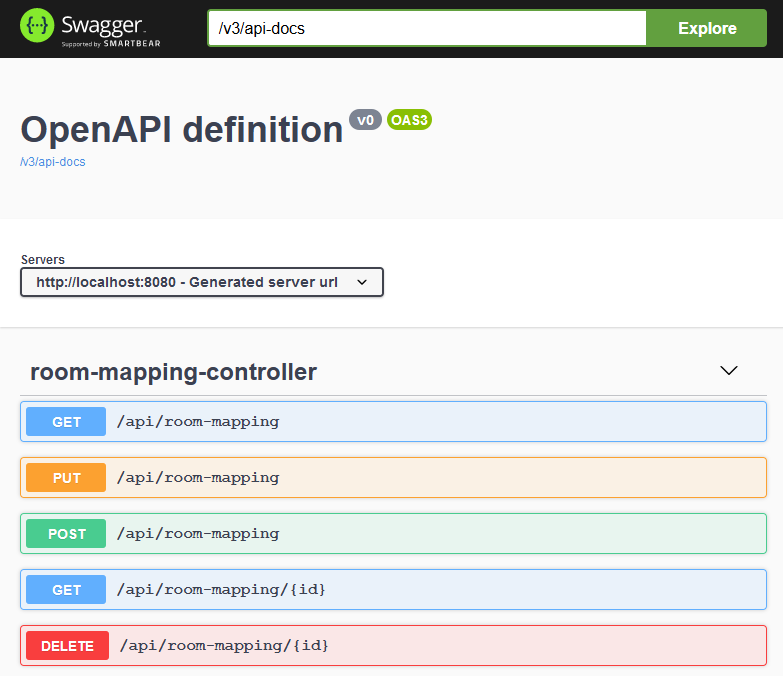
\includegraphics[width=0.5\textwidth]{res/screenshot-docs.png}
    \caption{Screenshot der dynamisch generierten REST-API Dokumentation, welche unter \texttt{api/documentation.html} verfügbar ist.}
    \label{fig:screenshot-docs}
\end{figure}

An dieser Stelle verzichten wir auf eine detailliertere Dokumentation der REST-API und einer Beschreibung der Objekte, da diese sich im Laufe zukünftiger Entwicklungen wahrscheinlich ändern werden.
Als Alternative stellt die Serveranwendung eine dynamisch generierte Dokumentation in Form einer Webanwendung unter \texttt{api/documentation.html} bereit wie sie in Abbildung~\ref{fig:screenshot-docs} dargestellt ist.
In der Dokumentation können neben den verfügbaren Schnittstellen die einzelnen Objektdefinitionen im JSON Format eingesehen werden.
Dabei ist anzumerken, dass die Definition für das \texttt{CADFile} Objekt nicht ganz korrekt ist.
In der Webanwendung der Dokumentation ist dort als Typ für das Attribut \texttt{data} \texttt{[string(\$byte)]} vermerkt, jedoch handelt es sich nicht um eine Liste von Zeichenketten, sondern lediglich um eine einzige Base64-kodierte Zeichenkette des CAD-Dateiinhalts.
Des Weiteren ist bei dem Attribut \texttt{charsetName} der Zeichensatz anzugeben, in welchem die Binärdaten der Datei kodiert sind, sollte es sich um eine Textdatei handeln (Beispielsweise \glqq{}utf-8\grqq{}).
Sollte es sich nicht um eine Textdatei handeln, der \texttt{type} also etwas anderes als das aktuell einzige unterstützte Format \texttt{dxf} sein, ist der Zeichensatz nicht mit anzugeben.

Weiter ist zu beachten, dass Attribute \texttt{id} und \texttt{createdTimestamp} der CAD-Datei- und Raumzuordnung-Entität generierte Werte sind.
So müssen diese nicht bei den \texttt{POST}-Methoden der REST-API mitgegeben werden, da sie vom Server bei der Erstellung zugewiesen werden.

Wir wollen abschließend noch kurz das Objekt der Raumzuordnung beleuchten.
Die restlichen Objektdefinitionen sind aus unserer Sicht intuitiv zu verstehen.
Die Raumzuordnung \texttt{RoomMapping} bezeichnet eine Zuordnung einer Kategorie zu einem einzelnen Raum.
Dabei können optional weitere Angaben, wie der Raumname oder eine Beschreibung mitgegeben werden.
Zur Zuordnung der Kategorie zu einem Raum können zwei Angaben gemacht werden: ein Mapping Vertex oder eine Liste von Vertices.
Es ist lediglich eine der beiden Angaben zu leisten um die Zuordnung durchführen zu können.
Bei Verwendung des Mapping Vertex versucht die Webanwendung später den Raum anhand eines einzelnen Vertex zuzuordnen, welcher sich auf der Kontur des Raums befinden muss.
Die Liste von Vertices kann alternativ verwendet werden, um eine genauere Zuordnung zu ermöglichen, wobei die einzelnen Vertices wieder auf der Kontur des Raums liegen müssen.
Die Raumzuordnungen werden in einer Sammel-Entität \texttt{RoomMappingCollection} für eine bestimmte CAD-Datei an die REST-Schnittstelle übermittelt.
Dabei ist die Reihenfolge der Raumzuordnungs-Objekte in der Sammel-Entität zu beachten.
Die erste Zuordnung in der Liste wird in der Webanwendung zuerst gezeichnet, die letzte zuletzt.
Sollten sich also mehrere Raumzuordnungen für denselben Raum in der Liste befinden, werden beide übereinander gezeichnet, wobei die letztere über die erste gezeichnet wird.

\subsubsection{Detailsicht der Webanwendung}
\label{subsubsec:detail-webapp}

\begin{figure}
    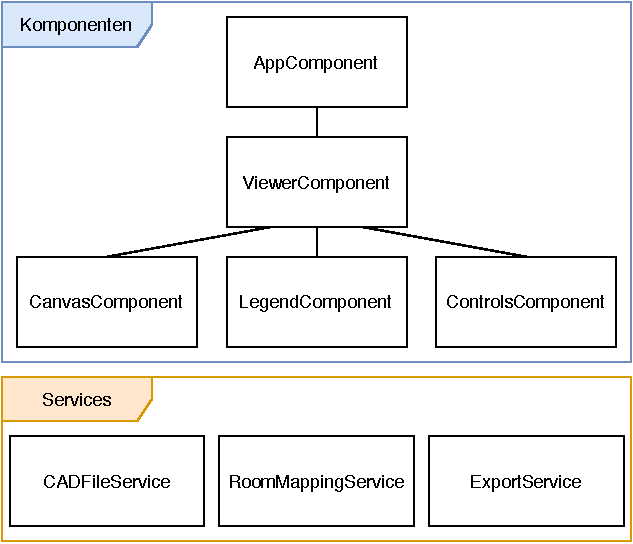
\includegraphics[width=0.5\textwidth]{res/frontend.pdf}
    \caption{Darstellung der wichtigsten Angular Komponenten und Services in der Webanwendung.}
    \label{fig:angular-components}
\end{figure}

Ein Blick zurück auf das Schaubild~\ref{fig:macro-view-diagram} zeigt die noch unbehandelte Webanwendung, die eigentliche Kern-Anwendung dieser Arbeit.
Dabei handelt es sich um eine Angular Anwendung, einem komponentenbasierten Framework.
Wir stellen die wichtigsten dieser Komponenten und einige ausgewählte Services in Abbildung~\ref{fig:angular-components} dar.
Services sind per \textit{Dependency Injection} in Komponenten verwendbare Objekte.
Meist werden darüber Komponenten übergreifende Funktionalitäten abgebildet, wie in unserem Beispiel die Kommunikation mit dem Server - etwa zur Verwaltung der CAD-Dateien.

Bei der \texttt{AppComponent} handelt es sich um die Einstiegskomponente in eine Angular Anwendung~\cite{AngularEntryComponent}.
Von dieser aus sind die anderen Komponenten in einer Baumstruktur dargestellt.
Eine Verbindung in Abbildung~\ref{fig:angular-components} bedeutet jeweils, dass die Komponente(n) unterhalb einer Komponente von dieser verwendet werden.

Die Wichtigste dieser Komponenten stellt die \texttt{ViewerComponent} dar, welche die eigentliche CAD-Viewer Anwendung implementiert.
Als Herzstück verwendet der Viewer eine \texttt{CanvasComponent} zum Zeichnen der Gebäudepläne.
Des Weiteren ist eine \texttt{ControlsComponent} zur Steuerung der Anwendung vonnöten, über welche Funktionen, wie das Öffnen einer CAD-Datei, zu jeder Zeit abgerufen werden können.

Wir wollen vor allem die \texttt{CanvasComponent}, also das Zeichnen der CAD-Dateien näher beleuchten.
Die Webanwendung unterstützt in der ersten Version nur DXF-Dateien, für welche in Abschnitt~\ref{subsubsec:comparison-parser-libs} bereits eine Parser-Bibliothek ausgewählt wurde.
Es ist jedoch vorstellbar, dass die Anwendung in Zukunft auch andere CAD-Dateitypen unterstützen soll.
Daher haben wir Vorkehrungen getroffen, um die Erweiterung möglichst einfach zu gestalten.
Wir stellen ein Interface \texttt{CanvasSource} bereit, welches der \texttt{CanvasComponent} als Quelle übergeben wird.
Es muss also lediglich eine neue \texttt{CanvasSource} für eine neuen Dateityp implementiert werden.
Dabei kann sich ein Beispiel an der bereits implementierten Quelle für DXF Dateien genommen werden.
Um den Vertrag des Interfaces zu halten, müssen zwei Methoden \texttt{draw} und \texttt{mapToRoom} umgesetzt werden.
Die Methode zum Zeichnen soll die verschiedenen Bestandteile der CAD-Datei auf eine \textit{three.js} Scene zeichnen.
Beispielsweise eine Linie muss so in eine für die Bibliothek \textit{three.js} geeignete Repräsentation umgewandelt werden.
In der \texttt{CanvasComponent} muss so lediglich das Zeichnen einer \textit{three.js} Scene unterstützt sein, unabhängig vom eigentlichen Typ der CAD-Datei.
Die \texttt{mapToRoom} Methode ist für die Raumzuordnung zuständig, also die Zuordnung von einem \texttt{RoomMapping} auf ein tatsächliches \textit{three.js} Objekt anhand der in der Raumzuordnung vorhandenen Attribute \texttt{mappingVertex} oder \texttt{vertices}.
Zwar ist die Zuordnung unabhängig vom CAD-Dateityp, allerdings ist es leicht vorstellbar, dass bestimmte Dateitypen anhand ihrer Metadaten den Mappingvorgang besser durchführen können (z. B. anhand des Raumnamens oder der Beschreibung).
Die Zuordnung wird im Abschnitt~\ref{subsubsec:room-mapping} im Detail behandelt.

Die \texttt{CanvasSource} ist nicht plötzlich vorhanden.
Sie muss beim Öffnen einer CAD-Datei erstellt werden.
Da dieser Prozess wieder vom Dateityp der CAD-Datei abhängig ist, gibt es ein weiteres Interface \texttt{CanvasSourceReader}.
Die Implementierungen für die verschiedenen Dateitypen werden in der Klasse \texttt{CanvasSourceReaders} in eine Hashmap gelegt und können per Dateityp geholt werden.
Beim Öffnen einer Datei wird ein geeigneter \glqq{}Leser\grqq{} aus der Map geholt und auf den Inhalt der CAD-Datei angewandt, was eine \texttt{CanvasSource} vom richtigen Typ zurückliefert.
Zusammenfassend ist die \texttt{CanvasComponent} vollständig unabhängig vom verwendeten Dateityp und erlaubt so eine einfache Erweiterung.

\subsubsection{Exportvorgang}
\label{subsubsec:export-process}

Nachfolgend wollen wir auf den verwendeten Exportvorgang eingehen.
Die Anwendung kann, wie bereits erwähnt, als HTML-Datei exportiert werden.
Dabei enthält die exportierte HTML-Datei die gesamte Webanwendung und zusätzlich die zur Zeit des Exports ausgewählte CAD-Datei und Raumzuordnung.

Die größte Herausforderung stellt hierbei sicherlich die Bereitstellung der gesamten Webanwendung als HTML Datei dar.
Normalerweise bestehen Webanwendungen aus vielen Dateien.
Vorstellbar sind beispielsweise Cascading Stylesheets, JavaScript-Dateien, HTML-Dateien, Bilder, Schriftarten und viele mehr.
Glücklicherweise gibt es bereits das Programm \glqq{}inliner\grqq{}, welches genau diese Aufgabe übernimmt und alle Ressourcen einer Webanwendung in nur eine HTML Datei verpackt~\cite{Inliner}.
Allerdings muss dafür die Webanwendung bereits mit einem HTTP Server bereitgestellt sein.
Daher modifizieren wir unseren Buildprozess dahingehend, dass bei jedem Build der Anwendung nun ein kleiner HTTP Server hochgefahren wird, die Webanwendung dort bereitgestellt, das Programm \glqq{}inliner\grqq{} eine HTML Datei erzeugt und der Server wieder heruntergefahren wird.
Die erzeugte HTML-Datei enthält nun die gesamte Export-Webanwendung und kann nun wie die ursprünglich gebaute Webanwendung von unserer Serveranwendung bereitgestellt werden.

Natürlich fehlen in der Export-HTML-Datei noch die CAD-Datei und die Raumzuordnung.
Daher gibt es die Export-REST-Schnittstelle in der Serveranwendung.
Die ID der zu exportierenden CAD-Datei und Raumzuordnung wird von der Webanwendung übermittelt.
Daraufhin wird die Export-Datei gelesen und die zusätzlichen Daten ergänzt.
Außerdem fügen wir eine zusätzliche \textit{globale} JavaScript Variable \texttt{app\_isExportMode = true} ein, welche der Webanwendung signalisiert, dass keine Verbindung zum Server hergestellt und stattdessen die eingebettete CAD-Datei und Zuordnung dargestellt werden sollen.
Die exportierte Datei kann so beispielsweise per E-Mail an andere Anwender geteilt werden, welche diese trotz fehlendem Server verwenden können.

\subsubsection{Raumzuordnung}
\label{subsubsec:room-mapping}

Ein weiteres Thema, das wir dokumentieren wollen, ist der Raumzuordnungs-Prozess.
Wir haben bereits behandelt, dass die vorhandenen Informationen zur Zuordnung die Attribute \texttt{mappingVertex} oder \texttt{vertices} der Raummapping Objekte sind.
Der einzelne Vertex sollte in den meisten Fällen ausreichen, um einen Raum korrekt zuzuordnen.
Voraussetzung dafür ist, dass die gegebene Koordinate nur auf der Kontur des zuzuordnenden Raums liegt.
Liegt die Koordinate auf mehreren Raumkonturen kann der Algorithmus keine eindeutige Aussage treffen.
Daher gibt es neben dem einzelnen Vertex auch die Möglichkeit mit dem Attribut \texttt{vertices} mehrere Vertices anzugeben.
Je mehr Vertices angegeben werden, die auf der Raumkontur liegen, desto wahrscheinlicher ist eine erfolgreiche Zuordnung.

Die Zuordnung an sich wird mehrstufig durchgeführt, um möglichst robuste Ergebnisse zu liefern.
Das bedeutet, dass verschiedene Methoden nacheinander versuchen die Zuordnung vorzunehmen.
Dabei ist die erste Methode das sogenannte \textit{Raycasting} mit \textit{three.js}.
Damit kann geprüft werden, ob Objekte sich mit einer gedachten Linie auf der \(Z\)-Achse (senkrecht zur Gebäudeplanebene) schneiden~\cite{Raycaster}.
Falls nur ein Vertex gegeben ist, wird das Raycasting für nur diesen Punkt durchgeführt.
Wird kein Ergebnis zurückgeliefert oder kein eindeutiges, ist die Zuordnung gescheitert.
Anders bei der Liste an Vertices: hier kann bei einem nicht eindeutigen Ergebnis der nächste Punkt probiert werden.
Schritt für Schritt werden so die Schnittpunkt-Objekte eliminiert, bis nur noch das Ergebnisobjekt der Zuordnung übrig bleibt.
Scheitert auch diese Methode wird ein Hashcode für die Liste an Vertices berechnet.
Dieser Hashcode wird als Schlüssel zum Lookup in einer Hashmap verwendet, welche bereits vorberechnete Hashcodes aller möglichen Räume vorhält.
Außerdem sind die vorberechneten Hashcodes bereits auf Objekte der Räume zugeordnet.
Diese Methode hat in unseren Experimenten gut funktioniert, allerdings unter der Voraussetzung, dass die Liste der Vertices genau der entspricht, die in der CAD-Datei vorliegen.
Daher befindet sich das Hashcode Mapping nur an zweiter Stelle in der Methodenliste.
Sollte auch die zweite Methode keine Zuordnung durchführen können, so nehmen wir an, dass die Liste an Vertices bereits einer ausreichenden Beschreibung des Raums entspricht.
Dementsprechend zeichnen wir auf Basis der Vertices ein Polygon über den Gebäudeplan.
Das hat den Nachteil, dass eventuell vorhandene Rundungen der Raumkontur nicht beachtet werden.
Allerdings können so auch indirekt Markierungen vorgenommen werden, die nicht unbedingt einem Raum entsprechen.
Beispielsweise ein Rechteck für einen Teil eines Raums.

Die bisher betrachteten Zuordnungsmethoden sind unabhängig von der CAD-Datei, allerdings nicht absolut zuverlässig.
Unglücklicherweise hat das DXF-Format keine weiteren Metainformationen zu einzelnen \glqq{}Entitäten\grqq{}, wie zum Beispiel Linien, zugeordnet.
Es ist allerdings vorstellbar, dass andere CAD-Dateiformate weitere Informationen bereitstellen und so beispielsweise eine Zuordnung anhand des Raumnamens ermöglichen.
